\chapter{Implementarea soluției}

Prin parcurgerea acestui capitol, cititorul va avea o imagine de ansamblu asupra modului în care senzorii sunt integrați în aplicație, cum este realizată comunicarea cu serverul și care sunt aspectele legate de programarea și funcționalitatea aplicației mobile. Aceste informații sunt esențiale pentru a înțelege arhitectura (Figura 3.1) și funcționalitatea aplicației în cadrul sistemului smart home propus.

\begin{figure}[h]
	\centering
	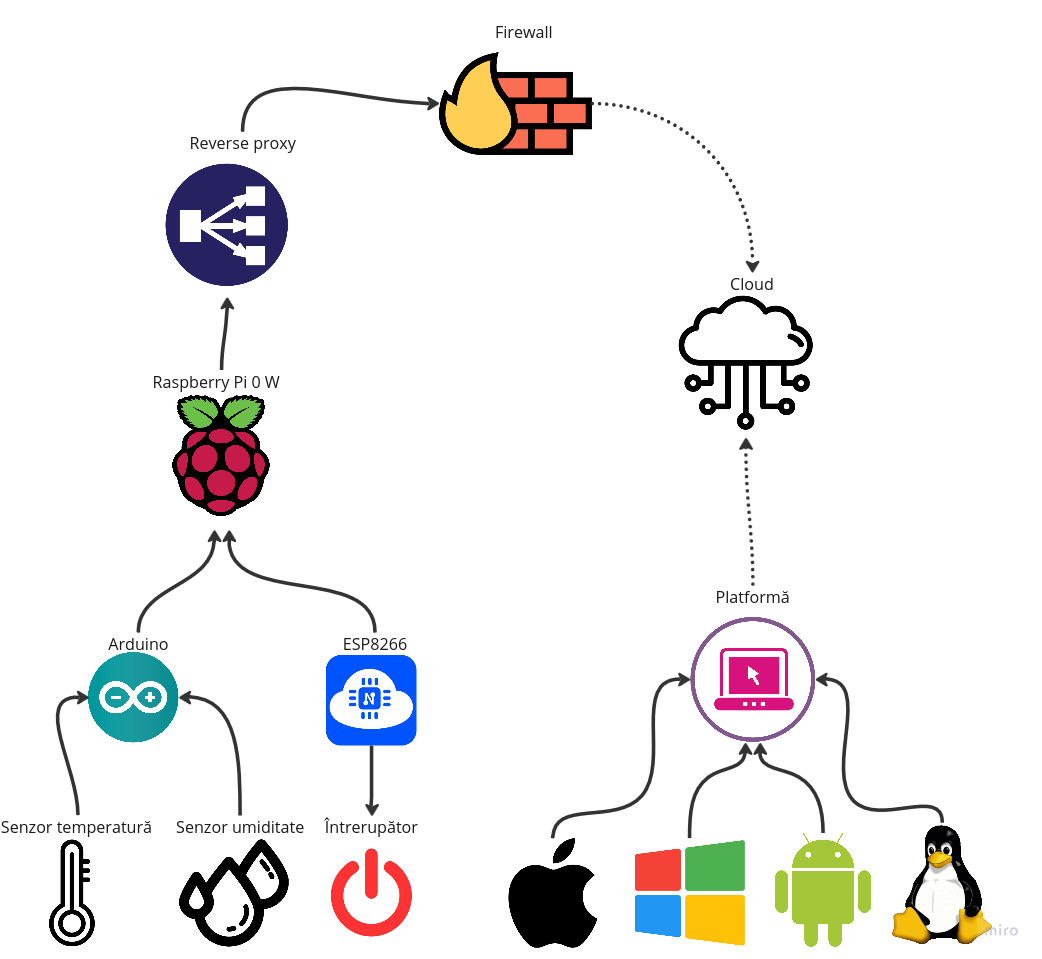
\includegraphics[width=1\textwidth]{arhitectura}
	\caption{Legătura dintre componentele soluției}
	\label{fig:arhitectura}
\end{figure}

INSERT C4 diagram

\section{Pagina principală}

\begin{wrapfigure}{r}{0.4\textwidth}
	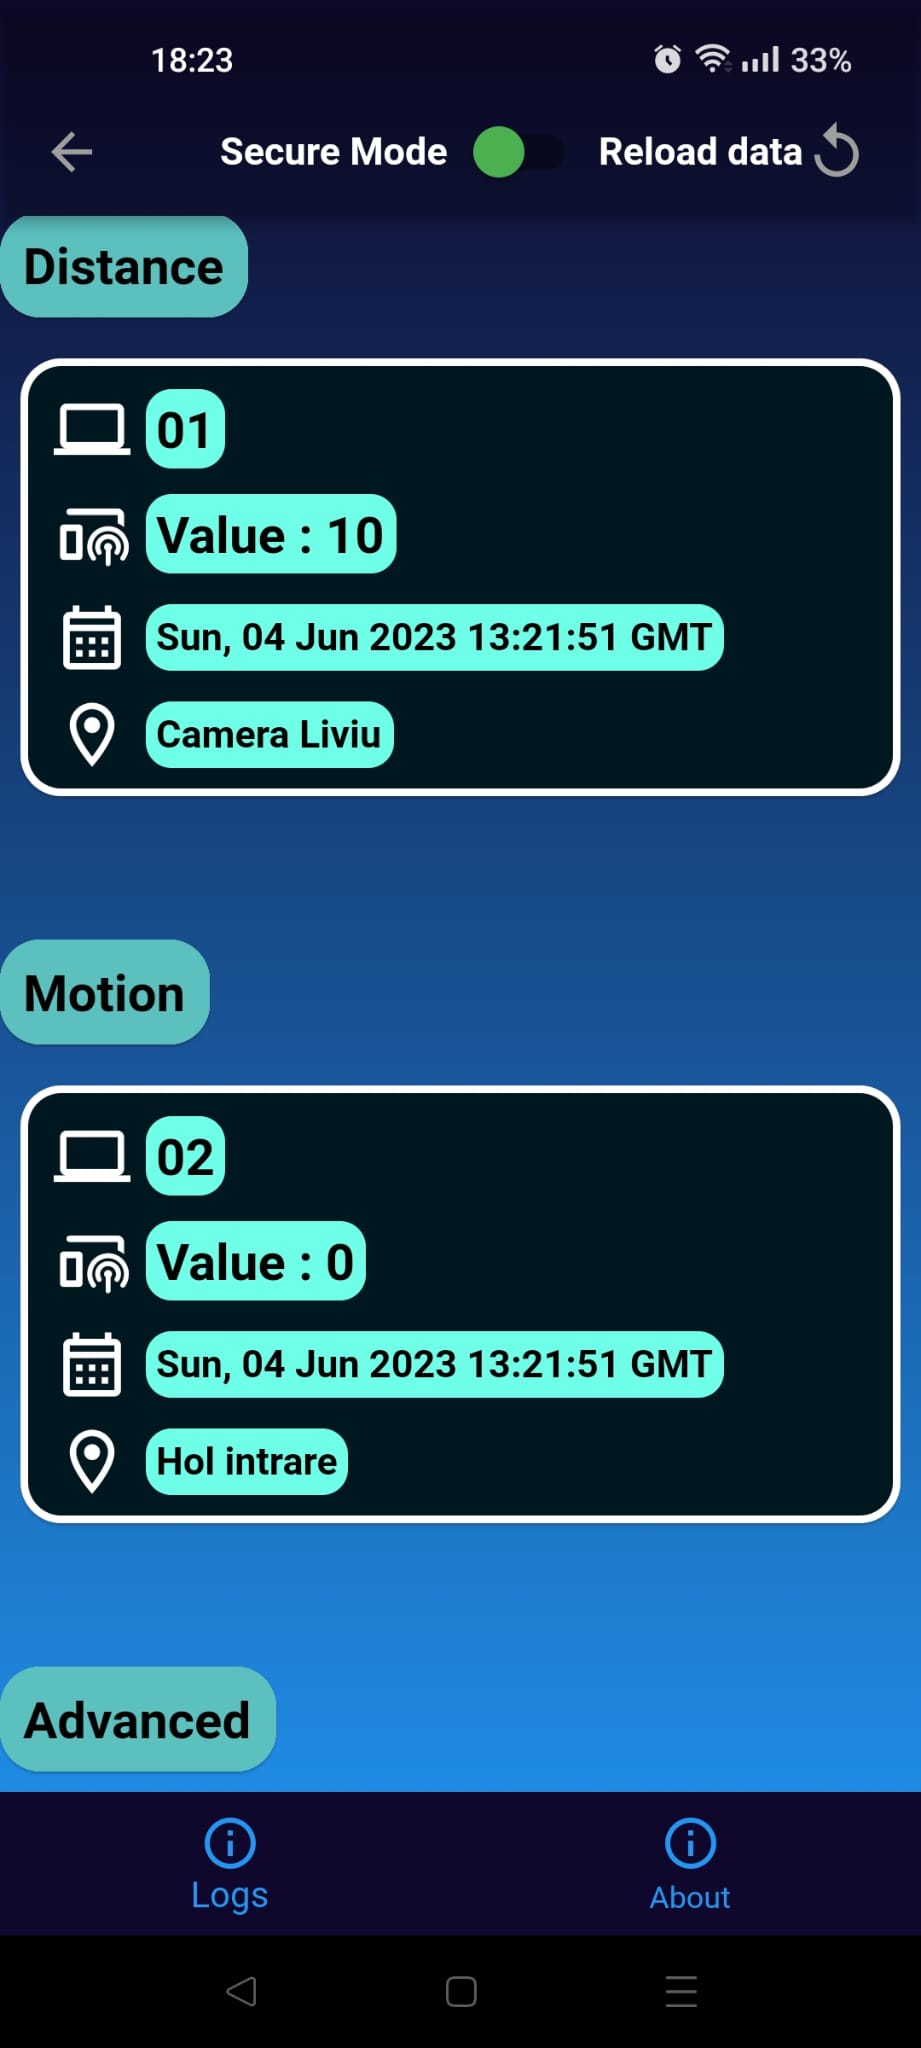
\includegraphics[width=1\linewidth]{1}
	\caption{Pagina principală}
	\label{fig:1}
\end{wrapfigure}

Primul punct de contact dintre un utilizator și acest proiect este aplicația de telefon (Figura 3.2). Odată lansată, va prezenta un splash screen, urmat de pagina principală. Aici se regăsesc toți senzorii conectați la sistem, împreună cu id-ul, valoarea cu timpul la care au fost înregistrate și locația din casă a senzorului. Aceștia sunt sortați după parametrul pe care îl colectează, fie detectarea mișcării, calcularea distanței, a temperaturii sau a umidității, lucru care se observă din titlurile situate deasupra fiecărui cartonaș. Aceste device-uri se numesc \emph{senzori statici}, secțiunea lor prezentând detalii despre modul de preluare și prelucrare a datelor. Mai există alt tip de senzor numit \emph{dinamic} a cărui caracteristici, din lipsă de spațiu vertical, vor fi explicate, asemeni celor de mai sus, în secțiunea lor.

În partea de sus se află două butoane, unul de activare/ dezactivare a \emph{modului de securitate} alături de cel de refresh care preia cele mai recente valori ale senzorilor, fiecare având o secțiune dedicată funcționalității și a modului de utilizare.

Pe post de footer sunt alte două butoane care servesc pe post de notificări atunci când valoarea unui senzor scade sub o anumită limită, respectiv cel de informații personale ale creatorului licenței.

\subsection{Cărțile senzorilor statici}

Cărțile reprezintă principala sursă de informații pe care un utilizator o regăsește instant când accesează aplicația. Ele oferă date importante despre senzorul respectiv într-o formă ușor de înțeles și de citit rapid.

În prima parte putem observa numele de identificare a senzorului. Acesta îi este asignat manual atunci când placa Arduino este programată și trebuie neapărat să fie unic în toată rețeaua. 
\begin{wrapfigure}{r}{0.4\textwidth}
	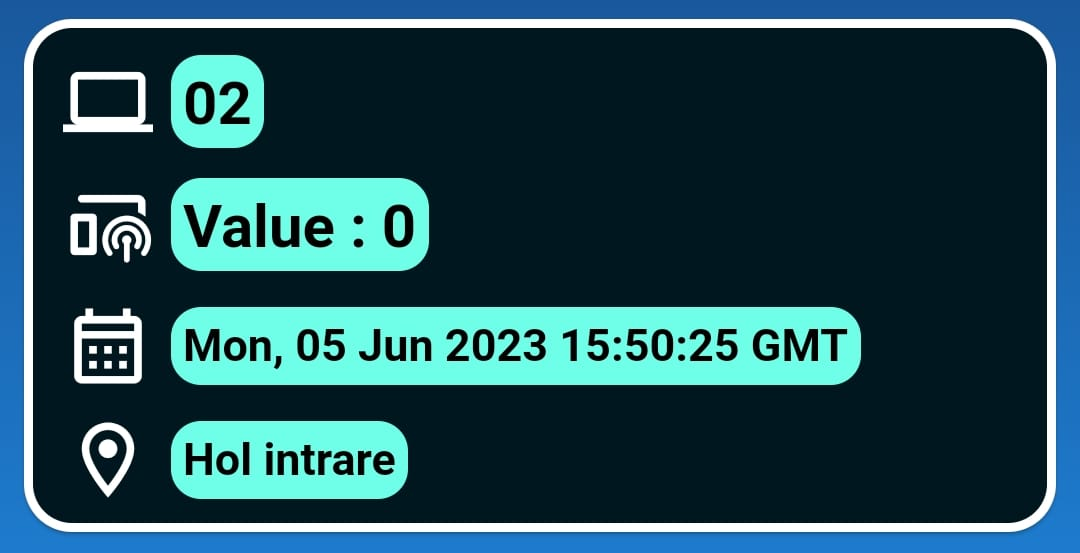
\includegraphics[width=0.5\textwidth]{3}
	\caption{Valorile unui modul}
	\label{fig:3}
\end{wrapfigure}
În cazul în care există multiple dispozitive cu același ID, stația de bază va crede că a primit două pachete de la același senzor, când defapt au fost trimise de către senzori care, foarte probabil, sunt programați să colecteze date diferite și astfel vor apărea discrepanțe vizibile între valorile trimise.

După, putem observa valoarea primită de către aplicație la data și ora respectivă. Odată ce este reîmprospătată pagina, dacă device-ul este conectat la rețea, telefonul va primi cea mai recentă măsurătoare din baza de date care primește informații noi odată la două secunde.

Și nu în ultimul rând, apare și locul fizic exact al senzorului, el fiind setat de către utilizator în aplicație. Inițial, acest câmp nu este vizibil deoarece senzorii nu au atașați un loc stabil, atașarea și schimbarea lui fiind făcute de către utilizator.
\subsection{Locația senzorului}

Cu un suport larg de diferite gesturi cu ajutorul clasei GestureDetector din Flutter, avem acces la o suită de detectări a mișcărilor degetetului care pot executa anumite funcții. În cazul aplicației, odată ce se ține apăsat pe un cartonaș, va apărea un dialog în care putem introduce locația fizică a senzorului.â

\begin{wrapfigure}{r}{0.4\textwidth}
	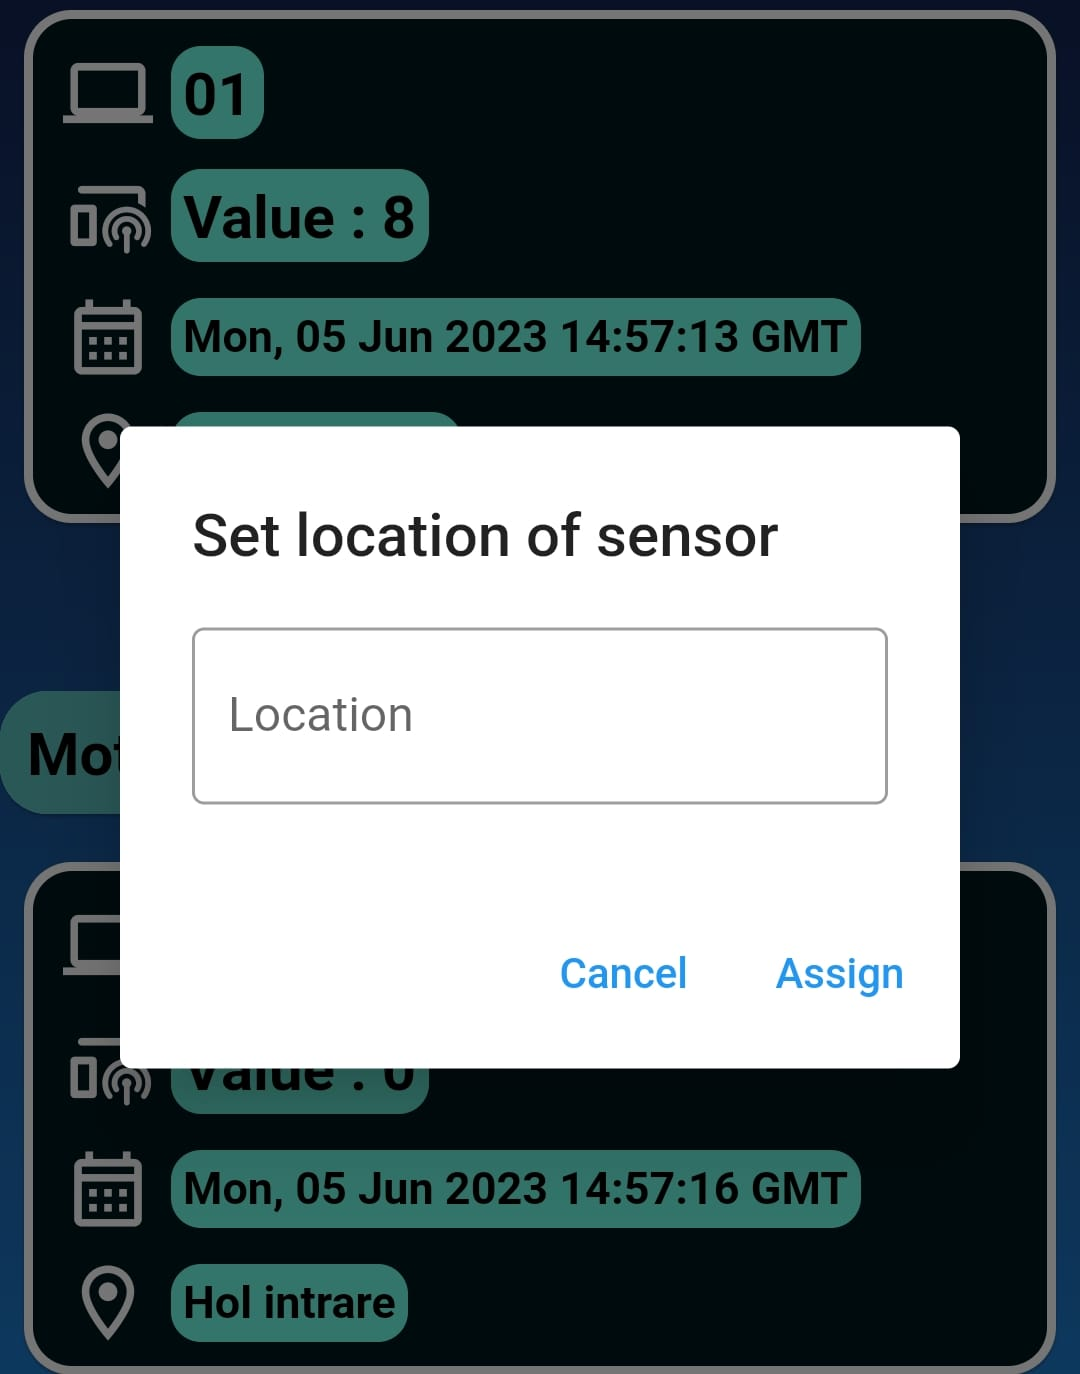
\includegraphics[width=0.5\textwidth]{2}
	\caption{Pop-up pentru locație}
	\label{fig:2}
\end{wrapfigure}

Aceasta este salvată în memoria locală a telefonului cu ajutorul bibliotecii de gestionare a bazelor de date NoSQL (non-relaționale). Am ales biblioteca respectivă datorită performanței ridicate, simplitatea oferită și compatibilitatea cross-platform care este critică deoarece aplicația aceasta poate fi compilată pentru majoritatea device-urilor populare. 


\section{Senzori statici}

Acest tip de device-uri stă la baza metodei de coletare a informațiilor despre casa respectivă și cea de generare a unui raport cu toate valorile din baza de date în intervalul cerut.

Figura 3.3.a ne prezintă cum a fost creat un senzor static: un Arduino Nano care este cablat la senzorul de detectare a mișcării și modulul de transmitere a datelor. 

Senzorul are 3 pini care trebuie conectați la placa de dezvoltare: Ground (împământare), Vcc (+5V) și Out. Ultimul pin emite un 0 logic dacă nu a detectat niciun obiect și 1 logic dacă a detectat o persoană sau un animal. Acest lucru este posibil datorită faptului că este emisă căldură în formă de radiații infra-roșii care alimentează componenta \emph{piroelectrică} (Figura 3.3.b) amplasată dedesubtul unei lentile Fresnel ce ajută focusarea acestor raze pe lentila senzorului. Modulul are încorporat două potențiometre: unul pentru reglarea razei de acțiune (până în 5 metri), iar celălalt pentru reglarea timpului de schimbare a valorii detectate (între 0.3 - 300 secunde). 

Odată alimentat la 5V, microcontroller-ul începe colectarea de date odată la două secunde. După ce acest interval a trecut, va fi creat un pachet ce conține ID-ul și tipul modulului, valoarea și data la care a fost făcută măsurătoarea. 

\begin{figure}[h]
	\centering
	\begin{subfigure}{0.85\textwidth}
		\centering
		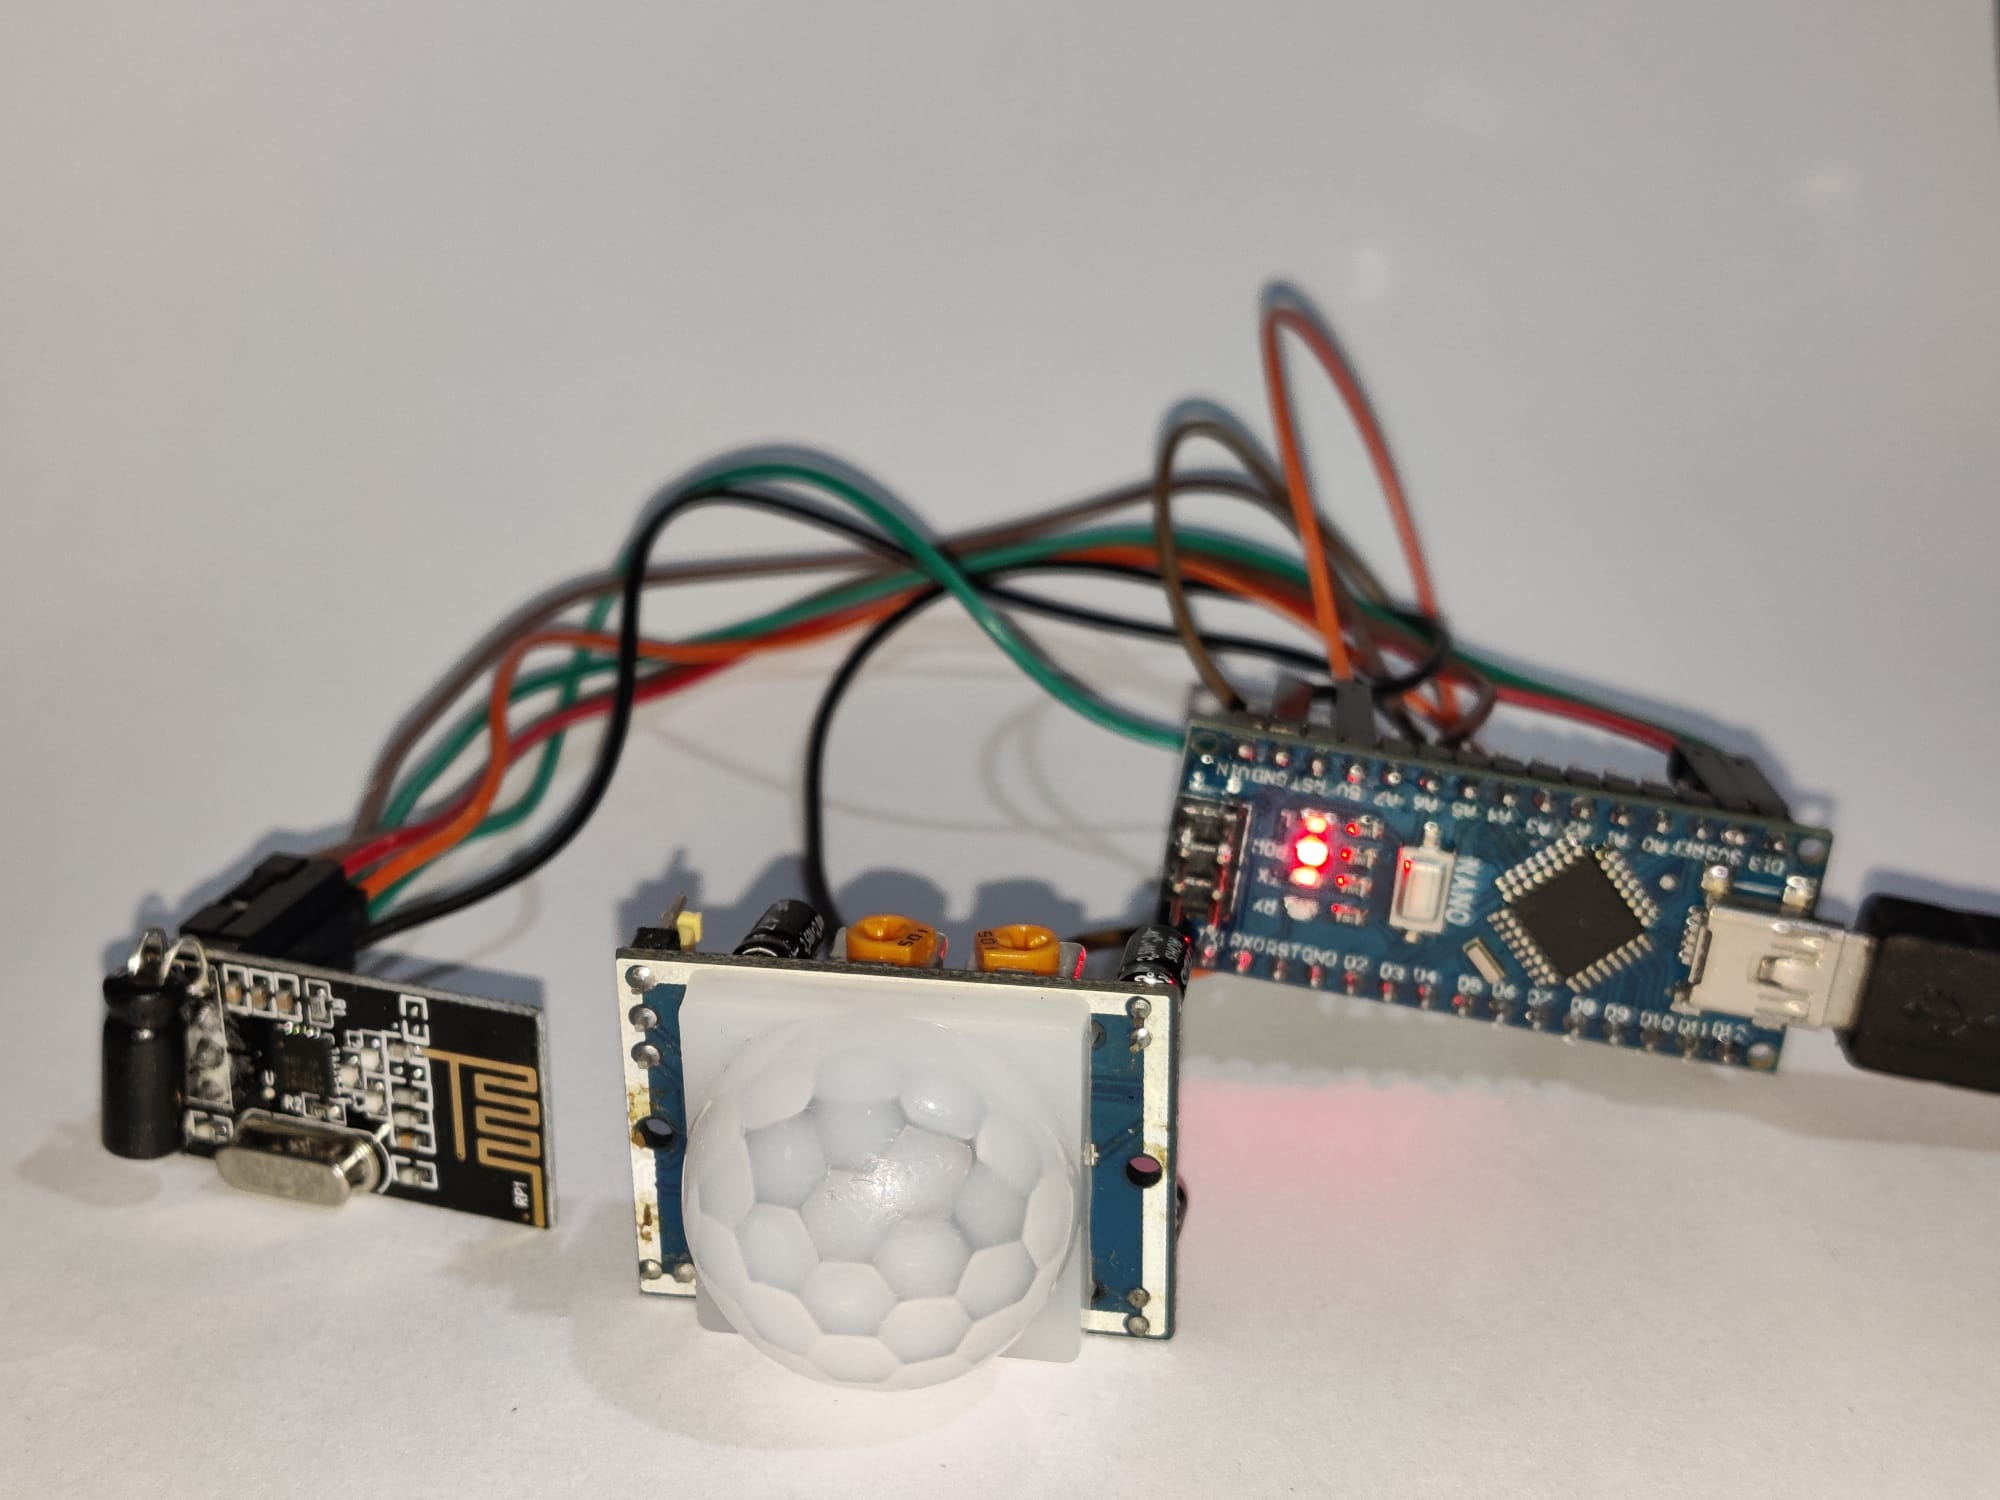
\includegraphics[width=0.8\textwidth]{static}
		\caption{Arduino Nano + senzor de mișcare + modul transmisie}
		\label{fig:static}
	\end{subfigure}
	\hfill
	\begin{subfigure}{0.8\textwidth}
		\centering
		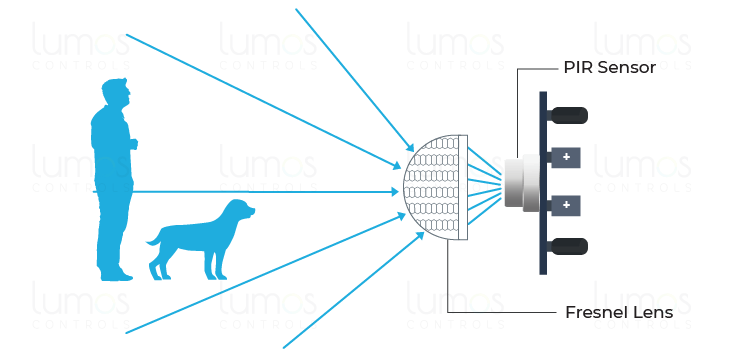
\includegraphics[width=0.8\textwidth]{pir}
		\caption{Componenta piroelectrică}
		\label{fig:pir}
	\end{subfigure}
	\caption{}
	\label{fig:all2}
\end{figure}
\break

Transmiterea și primirea acestor pachete va fi detaliată în secțiunea despre placa NRF24L01 unde vom vorbi de banda 2.4GHz, structura unui pachet de date și RF24Network. 

\section{Senzori dinamici}

Senzorii dinamici dețin o complexitate mai ridicată față de tipul anterior prezentat datorită faptului că pot trimite și primi date simultan de la server, făcându-i să pară că folosesc o conexiune \emph{full duplex}. Din cauza faptului că legătura dintre server și senzor se face prin intermediul protocolului Wifi, înseamnă că această legătură este mai degrabă \emph{half duplex}, schimbul de date realizându-se prin alternarea transmițătorului și receptorului, iar dispozitivele trebuie să respecte un anumit protocol de acces pentru evitarea coliziunilor și interferențelor cu alte dispozitive. CITAT

\begin{figure}[h]
	\centering
	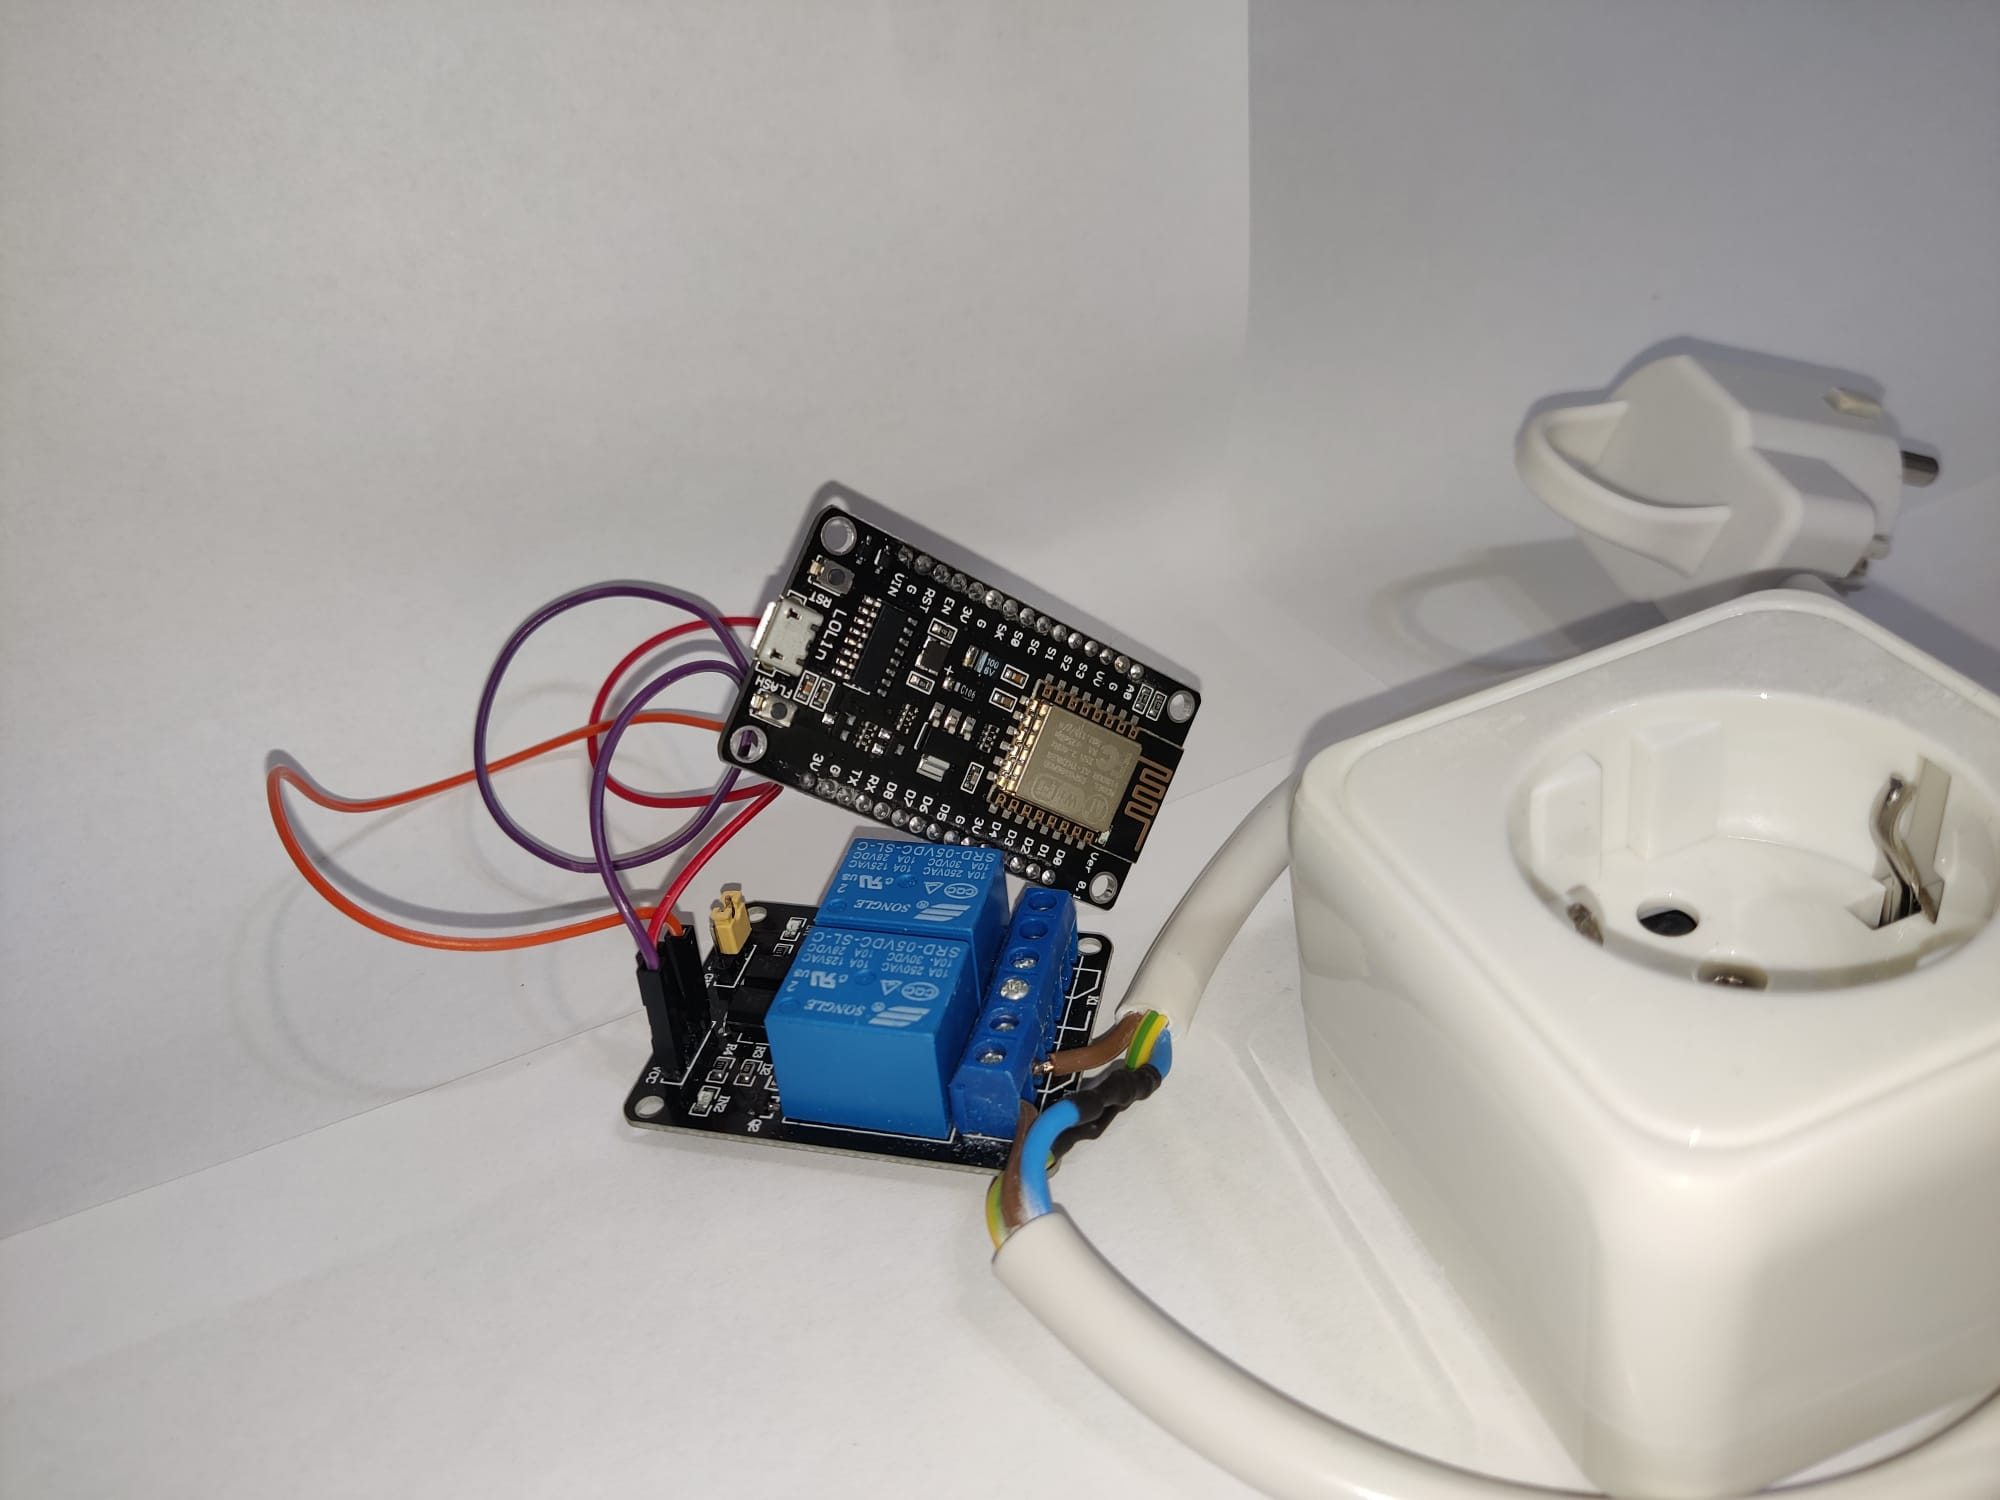
\includegraphics[width=1\textwidth]{dinamic}
	\caption{ESP8266 + modul releu alimentat la 220V}
	\label{fig:dinamic}
\end{figure}